% Name: Doppler effect
% Description: Wavefronts from a source moving right at half the wave speed: crowded ahead of it, where an observer hears a higher pitch, and spread out behind it.
% Tags: Doppler effect, wavefronts, frequency, sound

\usetikzlibrary{arrows.meta}

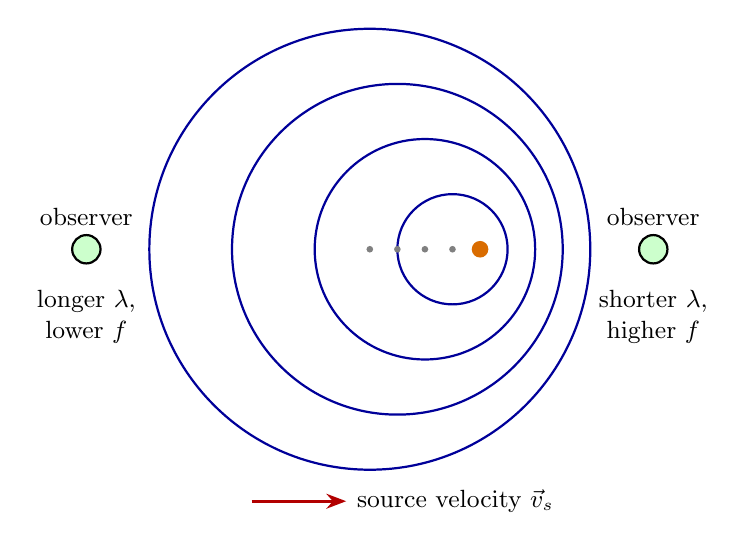
\begin{tikzpicture}[>={Stealth[length=2.5mm]}, every node/.style={font=\small}]
  % The front sent k seconds ago is centered where the source was then (x = -0.35k) with radius v k = 0.7k; ahead the fronts are 0.35 apart, behind 1.05.
  \foreach \k in {1,...,4} {
    \draw[thick, blue!60!black] ({-0.35*\k},0) circle ({0.7*\k});
    \fill[gray] ({-0.35*\k},0) circle (1.2pt);
  }
  \fill[orange!85!black] (0,0) circle (3pt);
  \draw[->, very thick, red!70!black] (-2.9,-3.2) -- (-1.7,-3.2) node[right, black] {source velocity $\vec{v}_s$};
  \draw[thick, fill=green!20] (2.2,0) circle (0.18) node[above=5pt] {observer};
  \draw[thick, fill=green!20] (-5,0) circle (0.18) node[above=5pt] {observer};
  \node[below, align=center] at (2.2,-0.4) {shorter $\lambda$,\\ higher $f$};
  \node[below, align=center] at (-5,-0.4) {longer $\lambda$,\\ lower $f$};
\end{tikzpicture}
